%%%%%%%%%%%%%%%%%%%%%%%%%%%%%%%%%%%%%%%%%%%%%%%%%%%%%%%%%%%%%%%%%%%%%%%%%%%%
%% Chapter 4
%%Indian Institute of Information Technology Kalyani
%% All rights are reserved.
%%%%%%%%%%%%%%%%%%%%%%%%%%%%%%%%%%%%%%%%%%%%%%%%%%%%%%%%%%%%%%%%%%%%%%%%%%%%
%
\chapter{Proposed Model for CBDC in India}
\label{chp4}

\section{Introduction}
As India moves rapidly toward a digital-first economy, the need for a robust and inclusive digital payment infrastructure becomes more necessary. Traditional systems, though effective, often fall short in addressing challenges like financial inclusivity, privacy concerns, and the ability to operate offline. To respond to these evolving demands, we propose a Central Bank Digital Currency (CBDC) model that is hybrid in nature—balancing centralized oversight with scalable, distributed access. This model is carefully designed with India’s diverse population, varied digital literacy levels, and dual online-offline payment needs in mind.

\section{System Architecture}

Our proposed CBDC system adopts a \textbf{hybrid architecture} that combines the central authority of the Reserve Bank of India (RBI) with the efficiency and reach of intermediaries such as banks and payment service providers. This layered approach enables regulatory control, promotes scalability, and ensures interoperability across platforms.

\begin{itemize}
    \item \textbf{Central Authority:} The RBI will be responsible for issuing the digital currency, integrating it with monetary policy, and maintaining the core digital ledger.
    \item \textbf{Intermediaries:} Licensed banks and payment service providers will handle distribution, wallet management, and user onboarding.
    \item \textbf{End Users:} Citizens can access and use CBDC through mobile apps, digital wallets, and even smart cards, depending on their preferences and connectivity.
\end{itemize}

\begin{figure}
    \centering
    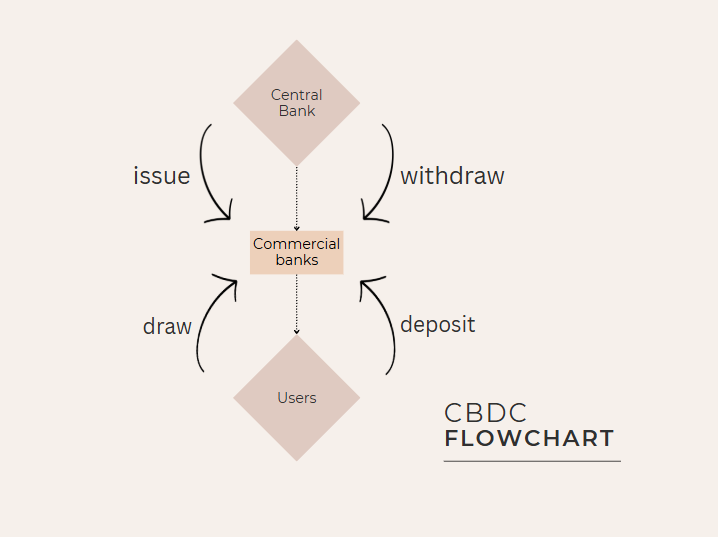
\includegraphics[width=0.8\linewidth]{image.png}
    \caption{Flow chart of CBDC architecture}
    \label{fig:enter-label}
\end{figure}
\begin{figure}
    \centering
    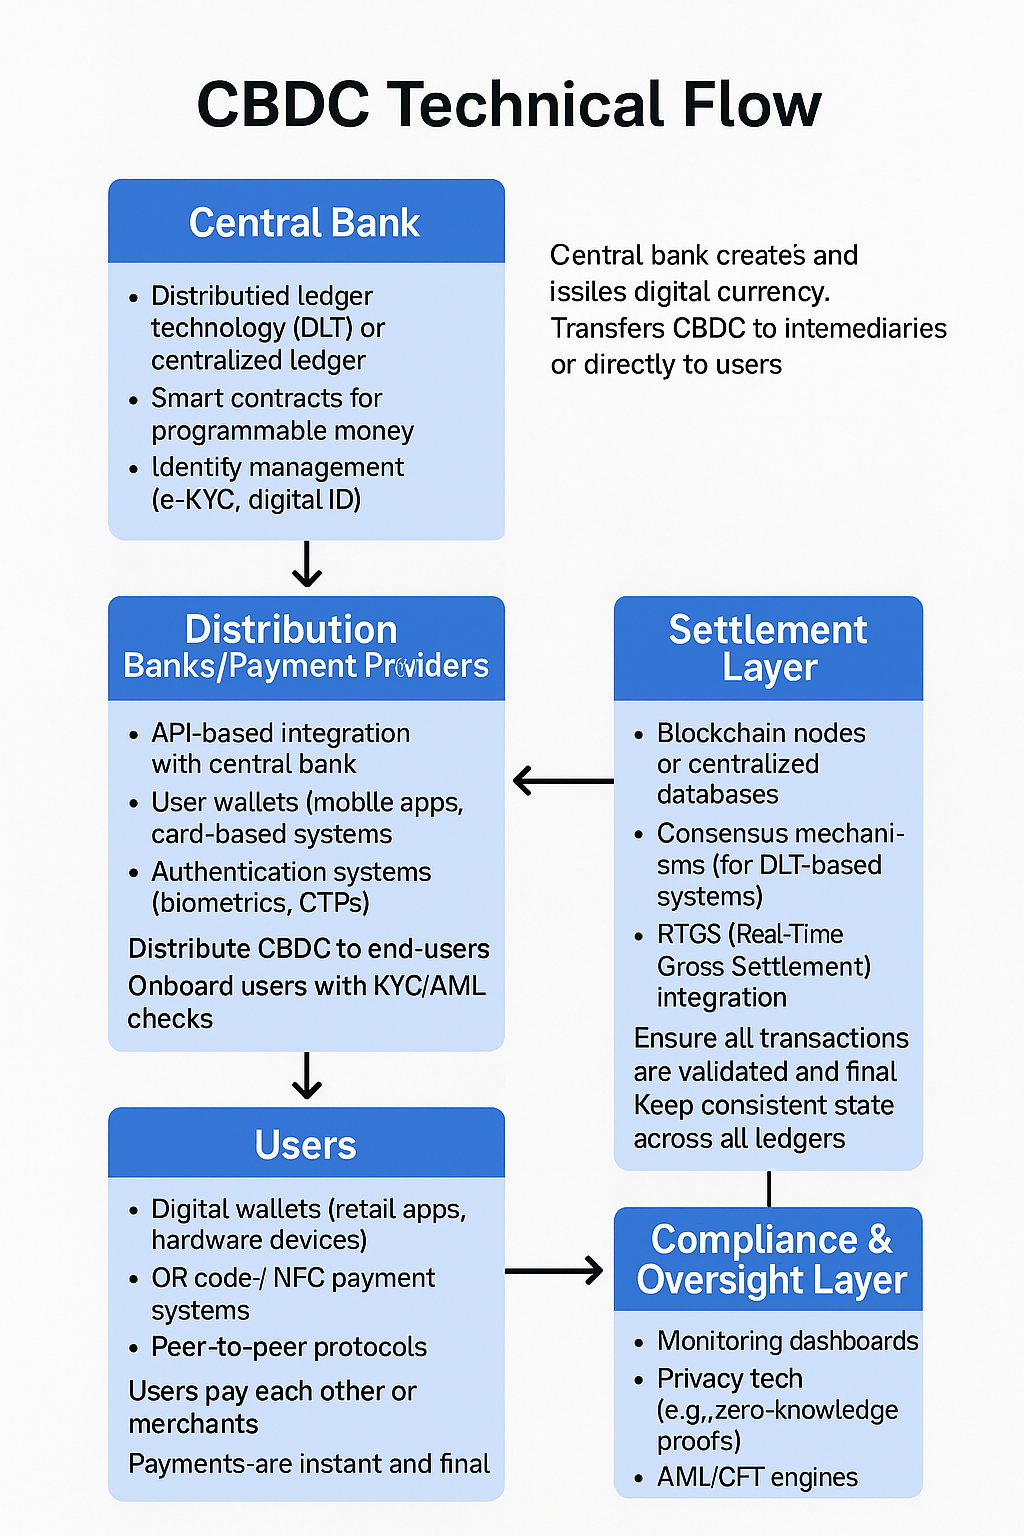
\includegraphics[width=0.8\linewidth]{image2.png}
    \caption{Proposed Architecture of CBDC for India}
    \label{fig:cbdc_architecture}
\end{figure}

\section{Ledger System}

The proposed CBDC architecture adopts a hybrid ledger model that brings together the strengths of both decentralized and centralized systems. At its core is a \textbf{permissioned Distributed Ledger Technology (DLT)}, designed to ensure that every transaction is secure, transparent, and efficiently recorded.

\begin{itemize}
    \item \textbf{Immutable Records:} Each transaction is cryptographically secured and permanently stored, ensuring data integrity.
    \item \textbf{Audit Trails:} The ledger maintains a complete and tamper-proof history of all transactions, which supports regulatory compliance and helps in detecting and preventing fraud.
    \item \textbf{High Scalability:} Optimized to handle millions of retail transactions in real-time, the system ensures smooth operation even under heavy load.
\end{itemize}

Alongside the DLT, the system also integrates a \textbf{centralized ledger} maintained by the Reserve Bank of India. This component plays a crucial role in managing monetary and regulatory functions efficiently.

\begin{itemize}
    \item \textbf{Central Oversight:} The RBI retains full authority over the issuance, distribution, and retirement of digital currency, ensuring policy control.
    \item \textbf{Policy Implementation:} Features like programmable money and interest-bearing CBDC can be implemented more seamlessly through centralized control.
    \item \textbf{Efficient Settlements:} High-value wholesale transactions can be settled quickly with reduced latency using centralized infrastructure.
\end{itemize}

This hybrid model strikes a balance between transparency and control—leveraging the innovation of distributed systems while preserving the central bank's ability to steer and supervise the financial ecosystem effectively.


\section{Token-based vs Account-based Models}

Given the diverse financial needs and digital maturity levels across India, the proposed CBDC model is designed to support both \textbf{token-based} and \textbf{account-based} approaches. This dual-model structure ensures flexibility, inclusivity, and alignment with varying use cases across the population.

\textbf{Token-based CBDC} operates much like physical cash in digital form. It is particularly well-suited for low-value transactions where privacy and ease of use are critical. Since ownership is validated through possession rather than identity, it allows for anonymous transactions, making it ideal for:

\begin{itemize}
    \item Peer-to-peer transfers in rural or underbanked areas.
    \item Offline payments where network access may be limited or unavailable.
    \item Small retail purchases where minimal friction and quick settlement are desired.
\end{itemize}

\textbf{Account-based CBDC}, on the other hand, functions similarly to a bank account. It requires identity verification and is directly linked to the user’s digital identity. This model is better suited for:

\begin{itemize}
    \item High-value or regulated transactions requiring KYC and AML compliance.
    \item Institutional and business payments where audit trails and accountability are necessary.
    \item Scenarios where programmable features or policy-driven restrictions (e.g., spending limits, taxation) are applied.
\end{itemize}

By integrating both models, the system accommodates a broad spectrum of users—from individuals seeking cash-like privacy to businesses and institutions requiring secure, regulated digital payments. This approach ensures that India's CBDC infrastructure remains inclusive, adaptable, and responsive to the evolving needs of its diverse economy.

\section{Stakeholders}

The success of the proposed CBDC ecosystem depends on seamless coordination among a range of stakeholders, each with a distinct and vital role. Together, they form an interconnected network that supports issuance, distribution, access, and everyday usage of the digital currency.

\begin{itemize}
    \item \textbf{Reserve Bank of India (RBI):}  
    As the sole issuer and regulator, the RBI oversees the creation, circulation, and overall governance of the CBDC. It ensures monetary policy alignment, sets operational guidelines, and maintains the integrity of the system.

    \item \textbf{Commercial Banks:}  
    Banks act as intermediaries between the RBI and end-users. They handle user onboarding through Know Your Customer (KYC) procedures, manage wallets and accounts, and facilitate the secure distribution of CBDC to individuals and businesses.

    \item \textbf{Payment Service Providers (PSPs):}  
    Fintech companies and digital wallet providers play a key role in delivering user-friendly platforms and mobile applications. Their focus is on enhancing user experience, enabling seamless retail payments, and ensuring broad accessibility—both online and offline.

    \item \textbf{Citizens and End Users:}  
    From tech-savvy urban professionals to rural individuals with limited digital exposure, citizens are at the heart of the CBDC ecosystem. Whether it's paying for groceries, sending money to family, or receiving government subsidies, the CBDC is designed to be intuitive and accessible for all.
\end{itemize}

By fostering collaboration across these stakeholders, the CBDC ecosystem ensures trust, efficiency, and inclusiveness—creating a foundation for a modern, digital economy that serves the entire population.

\section{Interoperability}

To ensure seamless integration with India’s current payment infrastructure, the CBDC is designed to work with:

\begin{itemize}
    \item \textbf{UPI, NEFT, RTGS:} For instant or scheduled transfers.
    \item \textbf{Wallets and POS:} Allowing both merchants and consumers to adopt CBDC without disruption.
\end{itemize}

\begin{figure}
    \centering
    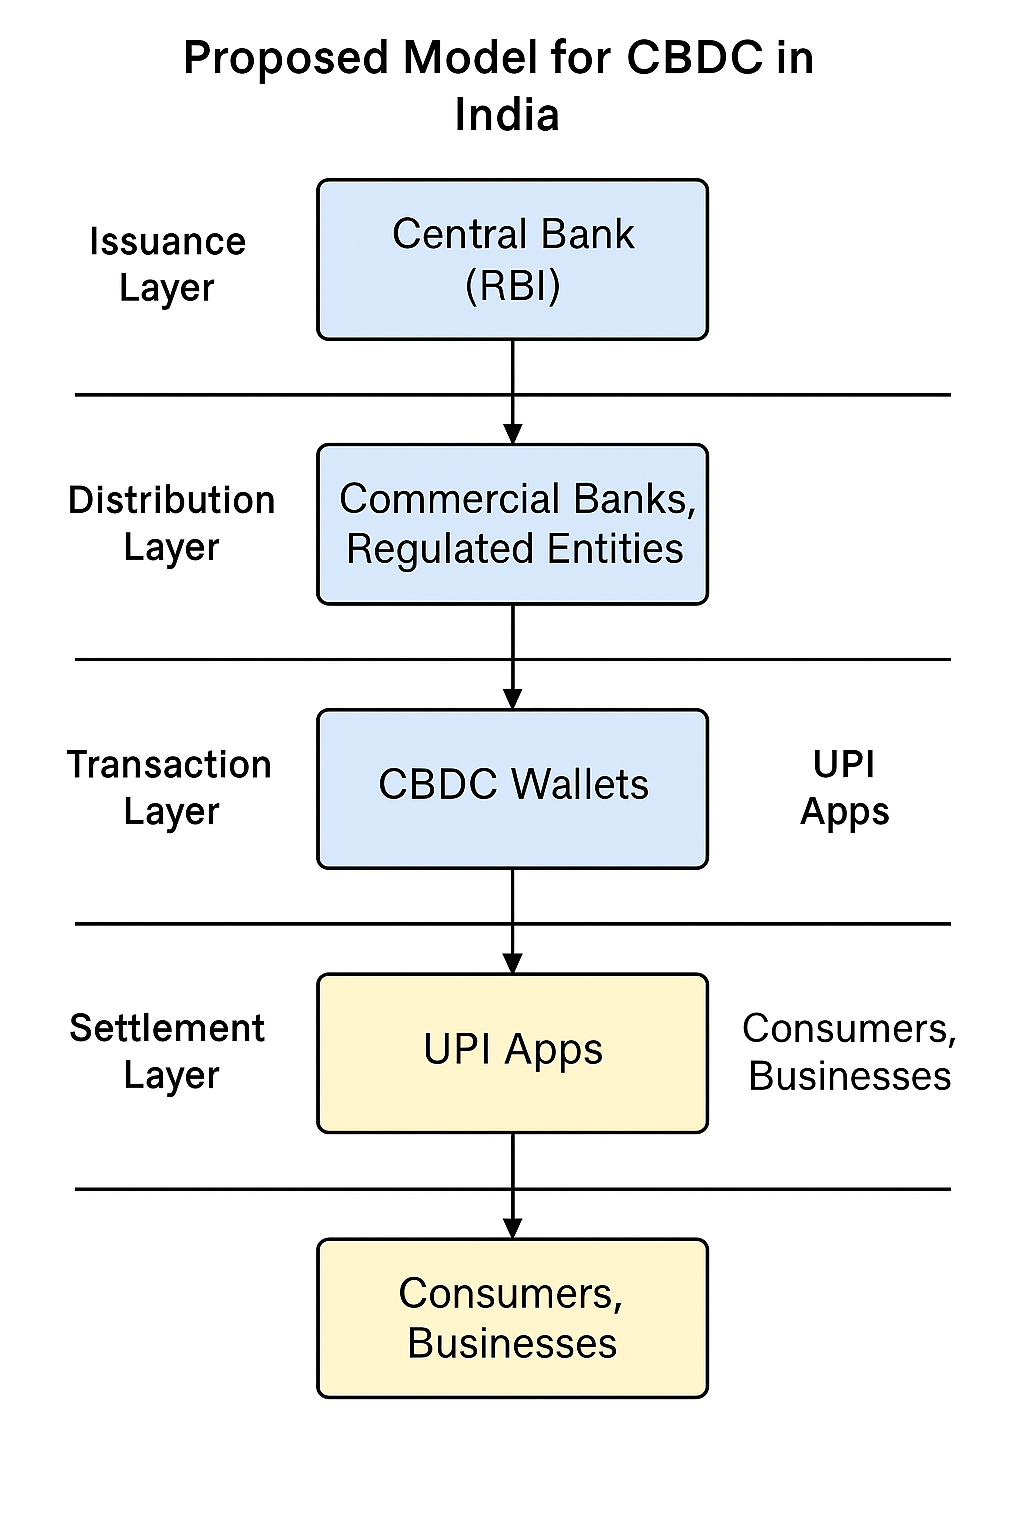
\includegraphics[width=0.75\linewidth]{image3.png}
    \caption{Flow chart of the model}
    \label{fig:enter-label}
\end{figure}
\section{Offline Capability}

One of the major strengths of this model is its ability to function even in areas with poor connectivity. Offline CBDC access can be enabled via:

\begin{itemize}
    \item \textbf{NFC-enabled smart cards}
    \item \textbf{QR code-based wallet apps}
    \item \textbf{Bluetooth-based peer-to-peer payments}
\end{itemize}

\section{Privacy and Security}

Security and privacy are built into the system through a \textbf{tiered KYC framework}, offering different levels of anonymity based on transaction size and use-case.

\begin{itemize}
    \item \textbf{Low-value transactions:} Allow pseudonymous access, preserving user privacy.
    \item \textbf{High-value payments:} Require full KYC and digital audit trails.
    \item \textbf{Advanced privacy tools:} Such as Zero-Knowledge Proofs (ZKPs) can be incorporated for enhanced confidentiality.
\end{itemize}

\section{Smart Contract Support}

To future-proof the CBDC system, the architecture supports smart contracts, enabling programmable financial tools such as:

\begin{itemize}
    \item \textbf{Time-bound payments:} Automatically revoke unclaimed subsidies after a deadline.
    \item \textbf{Conditional transfers:} For government benefits tied to specific uses.
    \item \textbf{Escrow mechanisms:} For safer e-commerce and service transactions.
\end{itemize}
\vspace{-5mm}
\section{Summary}
In summary, the proposed hybrid CBDC model is thoughtfully designed to address the diverse and evolving needs of India's economy and its people. It emphasizes \textbf{inclusivity}, ensuring that individuals across all regions---urban or rural, digitally connected or offline---can access and use digital currency with ease. The model is \textbf{scalable}, capable of handling the high volume and complexity of transactions in one of the world's most populous nations, while remaining \textbf{secure} through advanced technologies such as permissioned distributed ledger systems and tiered identity verification.
By integrating the strengths of India’s existing financial infrastructure---such as UPI, mobile wallets, and traditional banking---with modern digital innovations like offline payments, tokenization, and smart contracts, this CBDC model enables a \textbf{smooth and practical transition} toward a digital monetary system. Importantly, it reinforces public \textbf{trust} by maintaining central bank oversight, ensures \textbf{financial accessibility} even in underserved communities, and protects \textbf{monetary sovereignty} by offering a public alternative to private cryptocurrencies.
Ultimately, this hybrid architecture lays the foundation for a \textbf{resilient and future-ready digital economy}, where public digital money coexists and interoperates seamlessly with current systems, empowering citizens, businesses, and the broader financial ecosystem.\\\\\\\\\\
\pagebreak
\cleardoublepage